%\section{Markov Transition Fields for Uneven Sampled Time Series}
\section{Image Representation for Unevenly-Sampled Time Series}

With the motivation of processing the complete measurements (transitions) without using a subset of them we propose a method that simplifies the representation of long time series with unevenly-sampled measurements. The proposed method generates a bi-dimensional matrix (image) of the \textit{semi-continuous} transitions of a time series. By taking advantage of the time information, we build a 2 channel image representation: one for the observations (measurements) and the other one for the timestamps.

\subsection{Problem Setup}
Consider a dataset $X = \{x^{(1)}, x^{(2)}, \ldots, x^{(L)}\}$, of $L$ input patterns $x$ distributed according to an unknown probability distribution $p(x)$.
These input patterns are vectors of variable length, $x^{(\ell)}= (x^{(\ell)}_1, x^{(\ell)}_2, \ldots, x^{(\ell)}_{T_{\ell}})$, where $x^{(\ell)}_t \in \mathbb{R}^1$ represent the $t$-th observation (i.e., measurements) of the \textbf{time series} $x^{(\ell)}$ of length $T_{\ell}$. Let $s^{(\ell)}_t$ be the timestamp when the $t$-th observation was obtained from $x^{(\ell)}$. 

%We focus on transit-shape objects domain, where $x^{(\ell)}$ corresponds to a light curve that may be associated to an exoplanet transiting its host star. Two examples of light curves are shown on Figure \ref{fig:lc_ex}.

%\begin{figure}[t!]
%    \centering
%    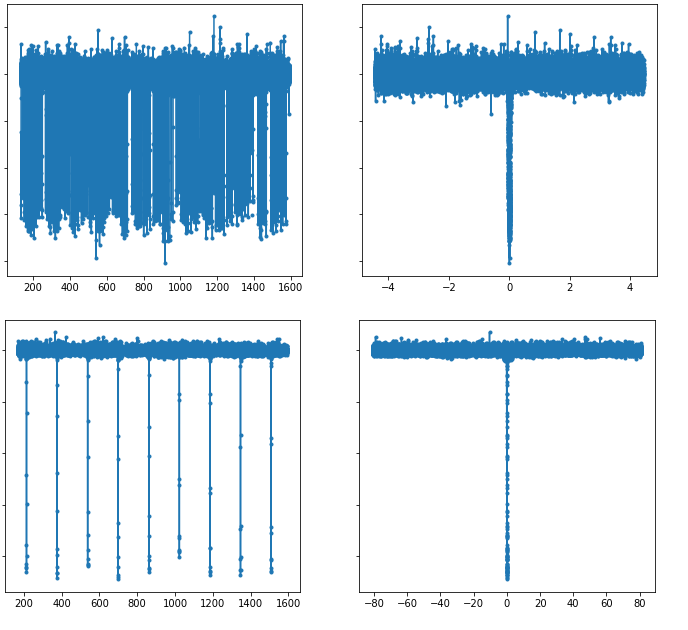
\includegraphics[width=0.95\textwidth, height=8cm]{imgs/LC_ex.png}
%    \caption{Examples of light curves on Kepler mission. First column correspond to 4 years measurements with sampling rate of half an our, while the second column correspond to the isolated transit.}
%    \label{fig:lc_ex}
%\end{figure}


%\subsection{Representation}

We assume that the time series measurements are median-centered and that the main variations are from the transients. Therefore, the values of interest are the negative transitions. We re-scale every light curve $x^{(\ell)}$ so that the $T_{\ell}$ measurements fall into $[-1,1]$ \citep{shallue2018identifying}. Based on the assumptions, the process is given by:
\begin{equation} \label{rep:pre}
    x_{t}^{(\ell)} = \frac{x_{t}^{(\ell)}}{min(x^{(\ell)})} \ , \ \ \forall t
\end{equation}


\subsection{Constructing the MTF}
\begin{algorithm}[!t] 
\caption{Light Curve to MTF}
\label{alg:lc_to_mtf}
\hspace*{\algorithmicindent} \textbf{Input}: $x^{(\ell)}$ - light curve measurements ($T_{\ell}$-dimensional vector) \\
\hspace*{\algorithmicindent} \hspace{0.1\textwidth} $s^{(\ell)}$ - light curve timestamp ($T_{\ell}$-dimensional vector) \\
\hspace*{\algorithmicindent} \hspace{0.1\textwidth} $n_{up}$ - number of states in positive values \\
\hspace*{\algorithmicindent} \hspace{0.1\textwidth} $n_{down}$ - number of states in negative values \\
\hspace*{\algorithmicindent} \hspace{0.1\textwidth} $\delta_T$ - maximum delta time \\ %tiempo pepe
\hspace*{\algorithmicindent} \textbf{Output}:  $M$ - MTF ($N \times N$ matrix)
\begin{algorithmic}[1]
\State $N \gets n_{up}+ n_{down}$  %N
\State $M \gets $ empty$(N, N)$
\State $S_{grid} \gets $ states\_grid$(n_{up},n_{down})$ \ //list of interval states
\For {observation $t \in \{1,2, \ldots, T_{\ell}-1\}$}
    \State $delta \gets s^{(\ell)}_{t+1}-s^{(\ell)}_t$
    %\If{$\mid  delta - \delta_T  \mid \leq \epsilon $ }
    \If{$  delta \leq \delta_T + \epsilon $ }
        %\State //Add state transitions count
        \State $i \gets $ detect\_state$(x^{(\ell)}_{t},S_{grid})$
        \State $j \gets $ detect\_state$(x^{(\ell)}_{t+1},S_{grid})$
        \State $M_{i,j} \gets M_{i,j} + 1$ \ //add state transitions count
    %\Else{}
    %    \State continue
    \EndIf
\EndFor
%\State 
\For {state $i \in \{1,2, \ldots, N\}$}  %N
    %\State $count_i \gets sum(M_{i,\cdot})$
    \State $M_{i,\cdot} \gets M_{i,\cdot}/ sum(M_{i,\cdot})$ \ //normalize probabilities  %   count_{i}$ 
\EndFor
\end{algorithmic} 
\end{algorithm}

%\documentclass[margin=0.5cm]{standalone}
%\usepackage{tikz}
%\usetikzlibrary{matrix,decorations.pathreplacing,calc,fit}

\pgfkeys{tikz/mymatrixenv/.style={decoration=brace,every left delimiter/.style={xshift=4.7pt},every right delimiter/.style={xshift=-4.7pt}}}
\pgfkeys{tikz/mymatrix/.style={matrix of math nodes, nodes in empty cells, left delimiter=[,right delimiter={]},inner sep=2pt,column sep=1em,row sep=0.5em,nodes={inner sep=0pt}}}
\pgfkeys{tikz/mymatrixbrace/.style={decorate,thick}}

% The hack required for foreach loops in fit. Code from https://tex.stackexchange.com/questions/4751/fitting-a-list-of-points-with-tikz-and-its-foreach?noredirect=1&lq=1
\makeatletter
\def\tikz@lib@fit@scan{%
  \pgfutil@ifnextchar\pgf@stop{\pgfutil@gobble}{%
    \pgfutil@ifnextchar\foreach{\tikz@lib@fit@scan@handle@foreach}{%
      \tikz@scan@one@point\tikz@lib@fit@scan@handle}}}
\def\tikz@lib@fit@scan@handle@foreach\foreach#1in#2#3{%
  \foreach #1 in {#2}
  {\tikz@scan@one@point\tikz@lib@fit@scan@handle@foreach@#3}
  \tikz@lib@fit@scan}
\def\tikz@lib@fit@scan@handle@foreach@#1{%
  \iftikz@shapeborder
    \tikz@lib@fit@adjust{%
      \pgfpointanchor{\tikz@shapeborder@name}{west}}%
    \tikz@lib@fit@adjust{%
      \pgfpointanchor{\tikz@shapeborder@name}{east}}%
    \tikz@lib@fit@adjust{%
      \pgfpointanchor{\tikz@shapeborder@name}{north}}%
    \tikz@lib@fit@adjust{%
      \pgfpointanchor{\tikz@shapeborder@name}{south}}%
  \else
    \tikz@lib@fit@adjust{#1}%
  \fi
  \global\pgf@xa=\pgf@xa
  \global\pgf@ya=\pgf@ya
  \global\pgf@xb=\pgf@xb
  \global\pgf@yb=\pgf@yb}
\makeatletter

%\begin{document}

\begin{figure}[!t]
    \centering
    %\includegraphics{}
    
\begin{tikzpicture}[baseline=0cm,mymatrixenv]
    \matrix [mymatrix,outer ysep=0.7pt,inner sep=4pt,row sep=1em] (m)  
    {
    m_{1,1}  &  m_{1,2} &  m_{1,3} & m_{1,4} & m_{1,5} &  m_{1,6} & \dots & m_{1,n}  \\
    m_{2,1}  &  m_{2,2} &  m_{2,3} & m_{2,4} & m_{2,5} &  m_{2,6} & \dots & m_{2,n}  \\
    m_{3,1}  &  m_{3,2} &  m_{3,3} & m_{3,4} & m_{3,5} &  m_{3,6} & \dots & m_{3,n}  \\
    m_{4,1}  & m_{4,2} & m_{4,3} & m_{4,4} & m_{4,5} & m_{4,6} & \dots & m_{4,n} \\
   m_{5,1}   & m_{5,2} & m_{5,3} & m_{5,4} & m_{5,5} & m_{5,6}  & \dots & m_{5,n} \\
    m_{6,1}  & m_{6,2} & m_{6,3} & m_{6,4} & m_{6,5}  & m_{6,6} & \dots & m_{6,n}\\
    \vdots   & \vdots  & \vdots  & \vdots  & \vdots  & \vdots  & \ddots & \vdots \\
    m_{n,1}  & m_{n,2} & m_{n,3} & m_{n,4} & m_{n,5} & m_{n,6} & \dots & m_{n,n} \\
    };

% Colours
\definecolor{brightpurple}{HTML}{C151EF}

\node [fit= \foreach \X in {1,...,3}{(m-\X-1)}
            \foreach \X in {1,...,3}{(m-\X-2)}
            \foreach \X in {1,...,3}{(m-\X-3)}]
            [draw=green, thick,inner sep=2.6pt] (fit-a) {};

\node [fit= \foreach \X in {4,...,6}{(m-\X-4)}
            \foreach \X in {4,...,6}{(m-\X-5)}
            \foreach \X in {4,...,6}{(m-\X-6)}]
            [draw=cyan, thick,inner sep=2.6pt] (fit-b) {};

\node [fit= \foreach \X in {2,...,4}{(m-\X-2)}
            \foreach \X in {2,...,4}{(m-\X-3)}
            \foreach \X in {2,...,4}{(m-\X-4)}]
            [draw=orange, thick,inner sep=2.6pt] (fit-c) {};
            
\node [fit= \foreach \X in {3,...,5}{(m-\X-3)}
            \foreach \X in {3,...,5}{(m-\X-4)}
            \foreach \X in {3,...,5}{(m-\X-5)}]
            [draw=purple, thick,inner sep=2.6pt] (fit-d) {};
            
% FINDING VERTICAL MIDPOINT
 \node [fit= \foreach \X in {1,...,3}{
            (m-\X-1)}] (fit-one)  {}; 
 \node [fit= \foreach \X in {4,...,6}{
            (m-\X-6)}] (fit-two)  {}; 
\path (fit-one.south) -- (fit-two.north) coordinate[midway] (X);

% FINDING HORIZONTAL MIDPOINT
 \node [fit= \foreach \X in {1,...,3}{
            (m-1-\X)}] (fit-one)  {}; 
 \node [fit= \foreach \X in {4,...,6}{
            (m-6-\X)}] (fit-two)  {}; 
\path (fit-one.east) -- (fit-two.west) coordinate[midway] (Y);

\newcommand\mymatrixbraceoffseth{0.3em}
\newcommand\mymatrixbraceoffsetv{0.3em}

% LHS BRACES
\draw [mymatrixbrace] ($(m.north west)!(fit-a.south)!(m.south west)-(\mymatrixbraceoffseth,0)$)   -- node[left=3pt] {$K_1$}  ($(m.north west)!(fit-a.north)!(m.south west)-(\mymatrixbraceoffseth,0)$);
\draw [mymatrixbrace] ($(m.north west)!(fit-b.south)!(m.south west)-(\mymatrixbraceoffseth,0)$) -- node[left=3pt] {$K_2$} ($(m.north west)!(fit-b.north)!(m.south west)-(\mymatrixbraceoffseth,0)$);

% TOP BRACES       
\draw[mymatrixbrace] ($(m.north west)!([xshift=0.05cm]Y)!(m.north east)+(0,\mymatrixbraceoffsetv)$) -- node[above=3pt] {$K_2''$}  ($(m.north west)!(fit-b.east)!(m.north east)+(0,\mymatrixbraceoffsetv)$);
\draw[mymatrixbrace] ($(m.north west)!(fit-a.west)!(m.north east)+(0,\mymatrixbraceoffsetv)$)-- node[above=3pt] {$K_1'$}   ($(m.north west)!([xshift=-0.05cm]Y)!(m.north east)+(0,\mymatrixbraceoffsetv)$);

\end{tikzpicture}
\caption{Illustration of a Markov Transition Field (MTF) matrix. Each entry into the matrix ($m_{i, j}$) corresponds to a defined state. Each box corresponds to a feature map for a $3 \times 3$ kernel size.}
\label{fig:matrix_MTF}
\end{figure}


%\end{document}

\begin{figure}[!t]
    \centering
    \subfloat[Light measurements transitions.]{{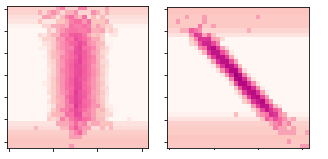
\includegraphics[width=0.45\textwidth]{imgs/MTF_lc_ex.png} }}%
    \qquad
    \subfloat[Time transitions.]{{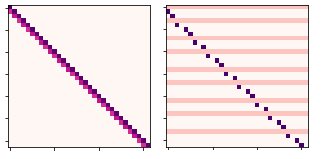
\includegraphics[width=0.45\textwidth]{imgs/MTF_time_ex.png} }}%
    \caption{Image representation (MTF) for light curve transitions (the measurements and the time) by using $n_{up}=n_{down}=16$ states ($32\times 32$ matrix). Examples are from light curves on the Kepler mission.}%
    \label{fig:mtf_ex:prop}
\end{figure}


A Markov Transition Field $M$ \citep{wang2015imaging} for a time series $x^{(\ell)}$ is constructed by taking all the continuous numerical values from $x_1^{(\ell)}$ to $x_{T_{\ell}}^{(\ell)}$. The meaning of a transition probability $m_{ij}$ in $M$ can be interpreted as the likelihood of transition from state $i$ to $j$ where $i,j \in N$. 
How to build this transition matrix for irregular sampled time series is not clear. We propose to take in consideration all the \textit{semi-continuous} (continuous over a maximum delta time) transitions to count the frequency and generate the probabilities with the relative frequency as \citep{wang2015imaging} propose. 
Thus, the probabilities $m_{ij}$ are built based on the number of \textit{semi-continuous} transitions from state $i$ to state $j$ (absolute frequency) normalized by the number of transitions from state $i$.
A pseudo-code to illustrate this for a $\ell$ time series is presented in Algorithm \ref{alg:lc_to_mtf}, where the main inputs are the measurements $x^{(\ell)}$ and timestamps $s^{(\ell)}$.
The maximum delta time to consider the \textit{semi-continuous} transitions ($\delta_T$) need to be defined too. It must be defined depending on the dataset behavior. In our case, we set it according the Kepler sampling rate (half of an hour).
%como conenctar con lo anterior??
First, we define a linear grid over the $[-1,1]$ interval to represent the states. We set different numbers for positive measurements $[0,1]$ (with $n_{up}$ values) and for negative measurements $[-1,0]$ (with $n_{down}$ values), this is the line 3 of the pseudo-code (i.e, ``states\_grid" function).
The number of intervals in positive and negative values could be manually defined in order to obtain more tailored transitions for each application while the ``detect\_state" function on line 7 and 8 finds the corresponding state for a specific measurement $x_t^{\ell}$ on the defined grid and
the line 6 is crucial, since it performs the \textit{semi-continuous} check of the transitions. 
Figure \ref{fig:mtf_ex:prop} shows examples of the final MTF matrix for the light curves observations.

Finally, $M$ has a dimension of $N \times N$, with $N=n_{up}+n_{down}$. In that sense, for convolutional neural networks \citep{krizhevsky2012imagenet}, a window of $k$ states represent the feature map that is fed to the model. So the feature map consider $k$ consecutive states from $M$, as Figure \ref{fig:matrix_MTF} shows.

%In addition, with the propose of use the irregular sampled time information, we build a time transitions matrix, described below.

\subsection{Constructing Time Transitions}
\begin{figure}[t!]
\centering
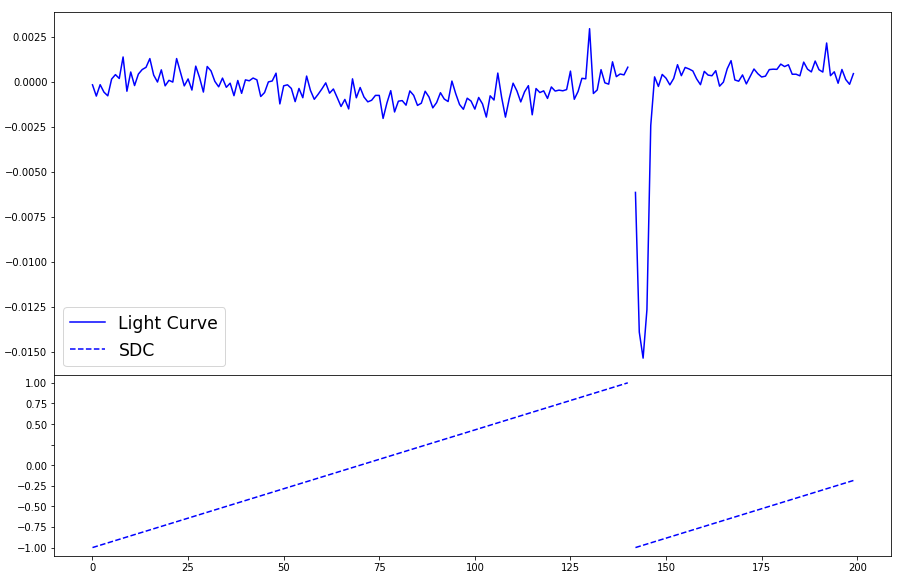
\includegraphics[width=0.85\linewidth, height=5cm]{imgs/sdc.png}
\caption{SDC from light curve. At the top image shows a sequence of 200 measurements from a given light curve; At the bottom is the SDC for the sample. Note that SDC is normalized in order to be consistent with the scale that the light curve has.}
\label{fig:sdc_example}
\end{figure}
To create the time channel for the image representation, we generate a \textit{Sample Detection Curve} (SDC) which maintains a sequence of counts of valid \textit{semi-continous} measurements based on a specific delta time, $\delta_T$. If two consecutive measurements have a timestamp difference greater than $\delta_T$, the count will restart. In this way, SDC provides information about the time transitions of a light curve. 
Algorithm \ref{alg:lc_to_sdc} shows how the SDC is build from the timestamps $s^{(\ell)}$ of a $\ell$ light curve considering a maximum delta time for \textit{semi-continuous} transitions ($\delta_T$).
Figure \ref{fig:sdc_example} shows a visual example of the SDC for a light curve.

\begin{algorithm}[t!] 
\caption{Light Curve to SDC}
\label{alg:lc_to_sdc}
\hspace*{\algorithmicindent} \textbf{Input}: $s^{(\ell)}$ - light curve timestamp ($T_{\ell}$-dimensional vector) \\
\hspace*{\algorithmicindent} \hspace{0.1\textwidth} $\delta_T$ - maximum delta time \\ 
\hspace*{\algorithmicindent} \textbf{Output}:  $SDC$ - semi continuous information ($T_{\ell}$-dimensional vector)
\begin{algorithmic}[1]
\State $SDC \gets empty(T_{\ell})$  //empty list of size $T_{\ell}$
\State $SDC[1] \gets 0$  //start of the sequence
\State $count \gets 1$
\For {observation $t \in \{1,2, \ldots, T_{\ell}-1\}$}
    \State $delta \gets s^{(\ell)}_{t+1}-s^{(\ell)}_t$
    \If{$\mid  delta - \delta_T  \mid > \epsilon $ }
        \State $count \gets 0 $ //reset count
    \EndIf
    \State $SDC[t+1] \gets count $
    \State $count \gets count + 1 $
\EndFor
\State $SDC \gets \frac{SDC - min(SDC)}{ max(SDC) -min(SDC)} $ // re-scale into [0,1]
\State $SDC \gets 2 \cdot SDC - 1$ // re-scale into [-1,1]
\end{algorithmic}
\end{algorithm}
Based on the re-scaled SDC (into $[-1,1]$ range) we can build the MTF of that information in the same way for light curve measurements.
The main idea is to apply Algorithm \ref{alg:lc_to_mtf} with the same number of states and maximum delta, but replacing the light curves measurements $x^{(\ell)}$ with the corresponding SDC.
Figure \ref{fig:mtf_ex} shows examples of the time channel on the final image representation (MTF), where it can be seen different sampling time patterns of the observation.



%\subsection{Number of States Effect}
%The number of states have a trade-off between a fine-grained (detailed) and a coarse (compressed) representation. A higher number of states will create a detailed fine-grained representation but sparser (with only a few transitions for each state). While a low number of state will group some states having a less detailed representation but denser (with more transitions for each state). Also it is complicated when it comes to define how many states on the positives ($n_{up}$) and on the negatives ($n_{down}$) values. For example, in order to have a more simpler and symmetric structure, we could define the same number of states for positive and negatives values. While if we want a matrix with more detailed transitions on the transits (blocking star light) the number of negatives states ($n_{down}$) has to be higher than the number of positives states ($n_{up}$). However, if we want a matrix with more detailed transitions on the out-of-shelf factors (e.g. background noise, astronomical objects or phenomenon) the $n_{up}$ value has to be higher than $n_{down}$.


